\begin{figure}[t]
  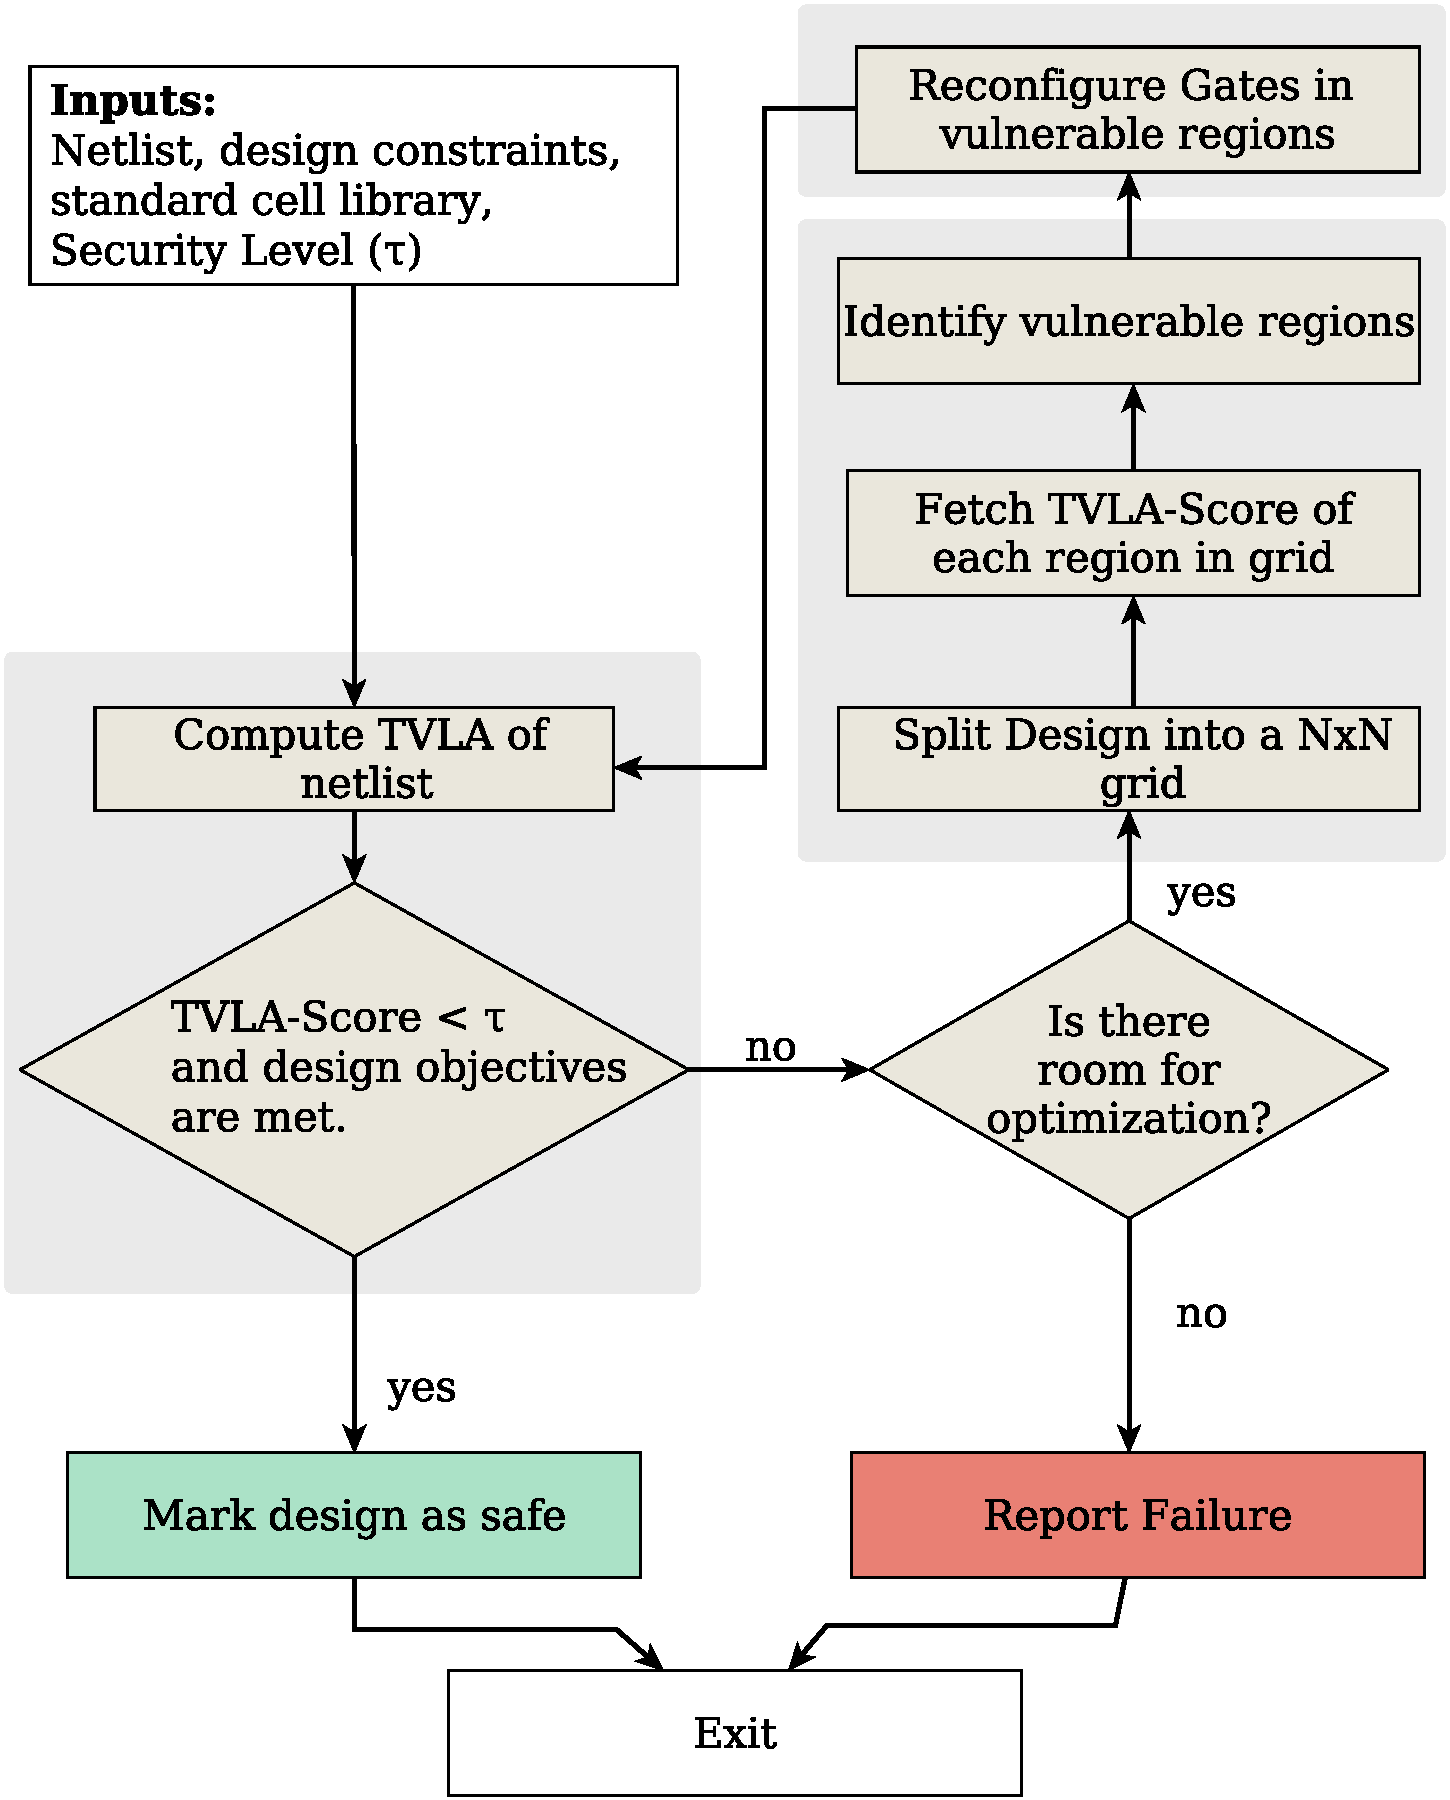
\includegraphics[scale=0.28]{Chapter4/karnamodule}
  \caption{Given a placed netlist, {\sf Karna} tries various configurations for gates present in the standard cell library until the required security $\tau$ is obtained.}
  \label{fig:proposed}
%  \vspace{-15pt}
\end{figure}

\section{{\sf Karna}: AN EDA Module to Reduce Side-Channel Leakage}
\label{sec:proposed}
The {\sf Karna} module (shown in Figure~\ref{fig:proposed}) is executed after the placement stage and before the routing stage in the EDA flow. {\sf Karna} takes as input the placed gate-level netlist represented as a directed acyclic graph $\mathbb C$, where the vertices are the gates and the edges represent interconnects. The various timing, power and area related information, obtained from the standard cell library, is then annotated to each node. Other inputs include $\mathbb P_{g}$, the set of all available choices for every gate type in the standard cell library, the target delay for the design D, and the user-specified security level specified as a desired TVLA score $\tau$.  

{\sf Karna} works in three steps. It first checks if the design meets the desired level of security $\tau$. If $\tau$ is not met, then {\sf Karna} divides the design into an $N \times N$ grid in order to identify the vulnerable regions in the grid. The algorithm then reconfigures the gates in these vulnerable regions until the desired level of security is achieved. We now discuss the implementation of the {\sf Karna} module in further detail. A detailed description is also specified in  Algorithm~\ref{alg:naive}.

{\flushleft \bf Estimating the side-channel security from the netlist.}
{\sf Karna} first estimates if the design meets the user-specified security level by performing the Test Vector Leakage Assessment~\cite{becker:2013} on the gate-level netlist (Line 1 in Algorithm~\ref{alg:naive}). For this, we select the input vectors as per the setup described in~\cite{becker:2013} and perform gate level simulation. The resultant switching information is recorded in a value change dump (VCD) file, that, along with the netlist, is given as an input to the power analysis tool available in the EDA flow. The tool  records the dynamic power traces for each gate in the netlist over a period of time. These traces can be used to compute the TVLA of the entire netlist as well as for specific regions in the netlist. If the TVLA of the design is less than $\tau$, the design passes the check and the algorithm exits successfully, otherwise {\sf Karna} proceeds to identify the vulnerable regions in the design.

{\flushleft \bf Identifying vulnerable regions.}
 {\sf Karna} uses Observation 2 (in Section~\ref{sec:motivation}) that, not all regions of the netlist contribute equally to the side-channel leakage. Hence, in order to reduce  side-channel leakage of a given design, it is sufficient for {\sf Karna}  to identify and optimize vulnerable regions in the netlist. Lines 2 to 12 in Algorithm~\ref{alg:naive} identify the vulnerable regions in the netlist. In order to do this, {\sf Karna} divides the netlist into an $N\times N$ grid and uses the dynamic power traces obtained in the previous step to compute the TVLA for each region $R$ in the grid. If the TVLA score for the region is greater than $\tau$, {\sf Karna} identifies gates that can be optimized by iterating through each gate in the selected region and adding them to a list $\mathbb W$. 
 A gate can be optimized if it meets the following conditions: {\em (i)} it can be replaced with its next low-power configuration {\em i.e.} if it has sufficient positive slack and, {\em (ii)} the gate is not critical. We define a gate to be critical if it cannot undergo any more reconfigurations. If there are no gates available, $\mathbb W = \emptyset$ (Line 13 in Algorithm~\ref{alg:naive}), and the algorithm reports failure and exits, otherwise, {\sf Karna} moves to the next step to reconfigure the vulnerable gates.
 
 




% \begin{framed}
% 1. Start with the flowchart and explain what each step is \\
% 	Explain the TVLA calculation step and how grid level tvla ties to the overall tvla score.\\
%     Explain that the grid can be customized. Explain why you divide into the grid \\
% 2. Explain the leakage optimization algorithm
% 3. Explain the optimization for placement (Need and algorithm)


% \end{framed}




\begin{algorithm}[!t]
%\algsetup{linenosize=\tiny}
  \scriptsize
  %\small
 \LinesNumbered
 \title{The {\sf Karna} algorithm}
 \caption{The {\sf Karna} algorithm}
 \label{alg:naive}
 \KwIn{The design $\mathbb C$ represented as a Directed Acyclic Graph, $\mathbb W$: the set of gates to be reconfigured,
 $\mathbb P_{g}$: the list of all possible configurations for gate g in increasing order of power, D: the delay constraint for the design and $\tau$: the user-specified security level.}
 
%\KwIn{Netlist of the given design C represented as a Directed Acyclic Graph (DAG), initial window size ($r_{init}$), upper bound on window size ($ry_{high}$), set of $V_t$,$V_{dd}$ and size for every gate sorted in increasing order of power, an array A containing the set of gates sorted by the TVLA score. }
\KwOut{Modified $\mathbb C$ so that the overall TVLA score is less than $\tau$.}

\While{$TVLA(\mathbb C) > \tau$}{
  \tcc{Identifying vulnerable regions}

$\mathbb W \leftarrow \emptyset $ \\
Divide the netlist $\mathbb C$ into $N\times N$ regions \\
%$\mathbb R_{regions} \leftarrow$ set of all regions \;
\For{each region $R$ in the  $N \times N$ grid}{
\If{$TVLA(R) > \tau$}{
\For{each gate $g$ in $R$}{
\If{$slack(g) > 0 $ and $g$ is not critical}{
$\mathbb W = \mathbb W \cup \{g\}$
}
}
}
}
\tcc{Reconfiguring vulnerable gates.}

\If{$\mathbb{W} \neq \emptyset$}{
Sort gates in $\mathbb{W}$ based on TVLA scores\\
\For{ each gate $g$ in $\mathbb W$} {
Let $\mathbb P_{g}[j]$ denote the current configuration of gate $g$\\
Let $\mathbb P_{g}[j-1]$ denote the next low power configuration of $g$\\

\If{$j==0$}{Mark $g$ as critical\\ \Continue}

\If{ $slack(P_{g}[j]) \geq delay(\mathbb P_{g}[j-1])-delay(\mathbb P_{g}[j])$  } {
Reconfigure g from $\mathbb P_{g}[j]$ to $\mathbb P_{g}[j-1]$ }
\Else { 
    Mark $g$ as critical\\
    \Continue }
Perform STA on $\mathbb C$ \\
\If{ $delay(\mathbb{C}) > D$}
{undo the reconfiguration done in Line 23\\
Mark $g$ as critical\\
\Continue
}
}
%Detect and fix slew and capacitance violations\;

}
\Else{
Report Failure and exit\;
}
}
%\If{$TVLA(\mathbb C) < \tau$}{
Report Success and exit\\
%Report Failure and quit\;
%}
% \If{No area violations}{
% Report Success and exit\;
 %
%
%
%
%

%%   $r = r_{init}$\; 
%   $state\leftarrow S_{11}$\;
%  $N \leftarrow gate\ count$\;
%   Run STA and compute slack for each gate\;
% % $sensitivity = $\nicefrac{ $\delta leakage \times slack $ }{$\delta delay \times paths$}$ $\;
%  A $\leftarrow$ list of gates whose TVLA score is greater \texttt{-security\_level} and have positive slack, sorted in descending order of sensitivity\; 
% %  \tcc{Note that all gates have slack value $\ge$ 0} 
%   \While{$A.size \ne 0$}  {
%     Take the top $r$ gates ($g_{k_1}, g_{k_2} \ldots g_{k_r}$) in $A$ \;
% %  \tcc{Local validation}
%      For each $g_{k_j}$ ($1 \le j \le r$), check if the increase in delay due to downsizing or upscaling of with its next $V_{dd}$, $V_t$ or $size$
%      version higher to its current version is lesser than its slack. If it is so, replace \;
% %  \tcc{Global validation}
%       Perform a full STA on C \;
%       If delay violation, undo all the reconfigurations done in step 8 \;
%       If $r=1$ mark gate $g$ as critical\;
%       Update the state as per Figure~\ref{fig:state-machine-window-sizing} \;
%       Update the value of $r$ as per Table~\ref{tab:window-sizing-strategy}, for the new value of state \;
%       Mark all the $r$ gates as replaced and remove from A\;
  %  }
 \end{algorithm}
% \begin{table*}[!ht]
%  \begin{minipage}{0.45\textwidth}
%  %\begin{center}
%  \centering

 %\scalebox{0.9}{

%  \begin{tabular}{|c|c|c|p{4cm}|c|}
%  \hline
%  State & $v_{i-1}$ &$v_i$ &Description &$r(i+1)\textsuperscript{*}$ \\
%  \hline
%  $S_{00}$ &0 &0 &Timing violation in the last two iterations& $1$ \\
%  \hline
%  $S_{01}$ &0 &1 &Timing violation in $(i-1)^{th}$ iteration and no timing violation in $i^{th}$ iteration& $(r(i))*2$ \\
%  \hline
%  $S_{10}$ &1 &0 &No timing violation in $(i-1)^{th}$ iteration and timing violation in $i^{th}$ iteration& $r(i) + \alpha$ \\
%  \hline
%  $S_{11}$ &1 &1 &No timing violation in the last two iterations& $r(i)^2$ \\
%  %\scalebox{0.9}{

%  \hline

%  \end{tabular}%}
%  \caption{The 2-bit prediction-based window sizing strategy adopted by {\it HALTimer}}
%  \label{tab:window-sizing-strategy}
%  %\end{center}
%  \end{minipage}\hfill
% %\begin{figure}[!ht]
% \begin{minipage}{0.35\textwidth}
%  \begin{center}
%  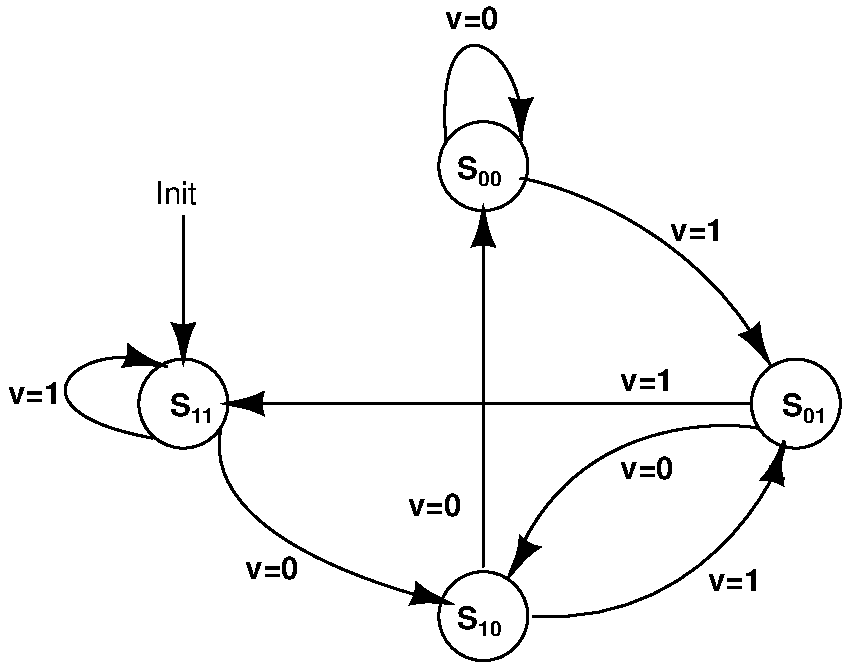
\includegraphics[scale=0.4]{fig/state_machine_window_sizing}
%  \captionof{figure}{Transition diagram for the 2-bit prediction scheme adopted by {\it HALTimer}}
%  \label{fig:state-machine-window-sizing}
%  \end{center}
% \end{minipage}
% \end{table*}






%{\sf Karna} works in three steps. First, it checks if the design meets the security requirement. If no, then it identifies the vulnerable regions and reconfigures the gate configurations in these regions. This process continues until the desired level of security is achieved. {\sf Karna} fails when either all gate configurations have been tried out or there is no more room for optimization. In this section we discuss the details of this process.

%\todo[inline]{fig 4. is it "Mark placement as safe" or "Mark netlist as safe"}

%takes as inputs the gate level representation of the design (gate-level netlist), the user specified security level, the standard cell library files, and $N_{grids}$. The parameter $N_{grids}$ specifies the number of grids the netlist must be divided into.  We now describe each steps in detail.
% \begin{figure}[!ht]
%  \centering
%   \includegraphics[scale=0.5]{fig/flow2.pdf}
%   \caption{The proposed flow. }
%   \label{fig:sub4}
% \end{figure}

%{\flushleft \bf Estimating the Side-Channel Security from the Netlist.} 
%For several input test vectors, {\sf Karna} performs a gate level simulation. The resulting switching information, stored in a value change dump (VCD) file, along with the gate-level netlist is given as an input to a power analysis tool, which records the dynamic power traces of each gate in the netlist over a period of time. These traces are then used to compute the TVLA~\cite{becker:2013} for the netlist. 
%If the TVLA score is less than $\tau$ then {\sf Karna} marks the netlist as safe and successfully exits. Otherwise, the next step is invoked which identifies the vulnerable regions in the design, 

%we divide the netlist into grid and use the power trace information to compute the TVLA score for each grid.
%Side-channel leakage of the design can be measured using a metric such as Test Vector Leakage Assessment (TVLA~\cite{becker:2013}). The required security level translates into the permitted TVLA score. If the TVLA score of the design  



%If the leakage from a particular grid is not within the limits specified by the user, the gates belonging to that grid are then reconfigured so as to reduce side-channel leakage. Subsequently, each gate in the vulnerable grid is reconfigured by optimizing one or more of the gate parameters such as supply voltage ($V_{dd}$), threshold voltage ($V_{th}$), load capacitance ($C_{load}$), and gate size. Modifying one or more of these gate-level parameters would impact the other design constraints. Therefore, we also verify that the area, power, and delay constraints are met. These operations are iteratively performed until the TVLA of every vulnerable grid in the design is within acceptable limits.

%The {\sf Karna} module takes as inputs the synthesized netlist which is a gate-level representation of the original design realized as per the design requirements realized at the synthesis step. In order to accurately esitmate the impact on the area constraint, the floorplan information, containting the location of each gate is passed via the def file. The module also takes as inputs the standard cell library which contains the power and delay information for each gate. The {\sf Karna} module lets the user specify the desired by the user by using the \texttt{-security\_level} option. The option specifies the TVLA score that the design is expected to meet. A lower TVLA score implies that the design is expected to meet strict security requirements while a higher score relaxes the security constraint for the design. 

%As mentioned in the previous section, the occurrence of side channel leakage is due to the presence of gates in the chip that perform differently when compared to that of a random input. The first step of the framework is to identify these vulnerable gates. The framework takes as inputs, the synthesized and placed verilog netlist, the floor-plan information and the library file. 

%We first check the post-placed netlist for the presence of side-channel leakage using the TVLA metric described in the Section~\ref{sec:background}.  If the netlist has an acceptable TVLA score, we stop the evaluation else if the netlist has the required TVLA score as specified by the \texttt{security\_level} option. If the design passes the module terminates and we proceed to the next step of the EDA flow. If a design fails to meet the desired level of security we then pass it to the next stage where the {\sf Karna } module identifies the vulnerable gates.


%\item 
% {\flushleft \bf Identifying vulnerable regions in the netlist.} 
%  This step uses the floorplan to divide the netlist into an $N\times N$ grid. {\sf Karna} then computes the TVLA score for each region in the grid using the same power traces estimated in the previous step. This is possible because \todo{fill up} If the TVLA score for a region exceeds the specified security level $\tau$ then that region is marked as unsafe. {\sf Karna} extracts all the gates in these unsafe regions that have a positive slack. The positive slack indicates that the gates can be reconfigured without affecting the delays of the design.  {\sf Karna} sorts these gates based on their TVLA and adds them to a list $\mathbb W$. It then reconfigures gates in the list {$W$}. This reconfiguration is discussed in the  next part of this section.
 
 
{\flushleft \bf Reconfiguring gates in unsafe regions.}
% \begin{itemize}
%     \item How we reconfigure gates such that power, delay, and area are not influenced. 
% \end{itemize}
We leverage Observation 3 (Section~\ref{sec:motivation}) that changing gate parameters has an impact on the overall side-channel leakage. {\sf Karna} optimizes gate parameters such that the overall security of the design improves while the design requirements like area, power, and delay remain unaffected. This reconfiguration is done in Lines 13 to 36 in Algorithm~\ref{alg:naive} by using a list $\mathbb P_{g}$ which contains all the possible configurations for gate $g$, sorted in the increasing order of power.
For each gate in $\mathbb W$, {\sf Karna} attempts to reconfigure it from its current configuration ($\mathbb P_g[j]$) to its next low power equivalent ($\mathbb P_g[j-1]$). However, doing so might compromise the design's delay constraint $D$. Hence, {\sf Karna} performs two validations: {\em (i)} a local validation, by checking if the reconfiguration does not violate the slack of the gate (Line 22) and {\em (ii)} a global validation by performing Static Timing Analysis (STA) for the entire design and checking if the arrival times at the outputs of the design do not violate the overall target delay  of the design $D$ (Line 30). The STA routine also checks for slew and capacitance violations and fixes them. If any of these constraints are violated, {\sf Karna} marks the gate as critical. A gate that is marked as critical is barred from taking part in any subsequent reconfiguration in the algorithm. 
The algorithm continues until the TVLA score drops below  $\tau$. This is a success and the result is a netlist $\mathbb C$, with gates suitably configured to meet the side-channel requirements of the design. The algorithm terminates with a failure if there is no room left for optimization. 


{\flushleft \bf An example with Simon.} 
A bit-serial implementation of the Simon block cipher\footnote{$https://opencores.org/projects/simon\_core$} requires 622 gates using a standard cell 28nm library. We identify the best possible delay of the design at 1.12ns and set it as the target delay $D$   and the desired security level $\tau$ is 4.5. We use 8000 inputs to perform TVLA analysis for the netlist $\mathbb C$, which we represent as a directed acyclic graph. In the first iteration of {\sf Karna}, the TVLA of the design is at 20.799 (Table~\ref{tab:simon}). 130 gates are identified as vulnerable as they belong to regions that have high TVLA ($< 4.5$). These gates are added to $\mathbb W$ as per Lines 4 to 12 in Algortihm~\ref{alg:naive}. The algorithm then attempts to reconfigure these gates as per the steps described in Lines 14 to 36. For the 28nm library used, each gate has 90 possible configurations. {\sf Karna} chooses suitable gates and then checks if the design meets $\tau$ by performing a second TVLA analysis. It can be seen that, after the first iteration, the TVLA of the design decreases to 10.83. This is still greater than $\tau$, which prompts  another iteration. The second iteration finds 102 vulnerable gates, which are  added to $\mathbb W$. Upon reconfiguring the gates {\sf Karna} once again, the TVLA score reduces to 4.48 which is less than $\tau$. The algorithm then exits successfully. 

\begin{table}[t!]
\scriptsize
\caption{Table showing the variation of TVLA, $\mathbb C$, $\mathbb W$, Delay and Power for the Simon cipher implementation in each iteration of Algorithm~\ref{alg:naive}. }
\label{tab:simon}
\centering
\begin{tabular}{|c|c|c|c|}
\hline
\textbf{}                                            & \textbf{\begin{tabular}[c]{@{}c@{}}$1^{st}$\\ Iteration\end{tabular}} & \textbf{\begin{tabular}[c]{@{}c@{}}$2^{nd}$\\ Iteration\end{tabular}} & \textbf{\begin{tabular}[c]{@{}c@{}}$3^{rd}$\\ Iteration\end{tabular}} \\ \hline
\begin{tabular}[c]{@{}c@{}}Delay\\ (ns)\end{tabular} & 1.12                                                                     & 1.12                                                             & 1.12                                                             \\ \hline
Power (uW)                                           & 3.70                                                                     & 2.61                                                             & 0.16                                                             \\ \hline
TVLA                                                 & 20.799                                                                   & 10.83                                                            & 4.48                                                             \\ \hline
$\mathbb C$ & \multicolumn{3}{|c|}{622}  \\ \hline
$\tau$ & 4.5 & 4.5 & 4.5 \\ 
\hline
$\mathbb W$ &       130 & 102 & 0 \\ \hline

\end{tabular}
\vspace{-10pt}
\end{table}

{\flushleft \bf Impact of {\sf Karna} on the other design requirements.}
{\sf Karna}, by design, does not violate the power and delay constraints. While the delay constraints are verified at multiple instances in the Algorithm~\ref{alg:naive} (Line 22 and Line 30), the power constraint is inherently met. This is because, {\sf Karna} attempts to replace each gate with its low power equivalents. Thus, the overall power consumption of the design will not increase.

While {\sf Karna} increases the area utilization of the device, it is unlikely to increase the  device size. The reason being, {\sf Karna} never adds any extra gates to the design but only reconfigures a targeted subset of the gates in the entire design. 
Not all the reconfigurations of these gates have an impact on the size. Further, the overall area would only increase if the gates lying at the periphery undergo an increase in size. There is low likelihood of this happening.


{\flushleft \bf Analysis of {\sf Karna}. }
We evaluate {\sf Karna} with respect to success and runtime.

{\flushleft \em Success Analysis.}
The success of {\sf Karna} depends on the value of $\tau$, the target delay of the design $D$, and the number of configurations available for each gate $|\mathbb P_g|$. A high value of $D$ implies that the slack at each gate will be high, thus, fewer gates will be marked critical. Consequently the number of gates taking part in the optimization process increases. Similarly, larger number of configurations available for a gate, will increase the chances that {\sf Karna} will find a gate which can achieve the desired security. A lower value of $\tau$ on the other hand, increases the effort that {\sf Karna} has to put in to achieve  security requirements. This may lead to an infeasible solution. 

\begin{figure}[t!]
\centering
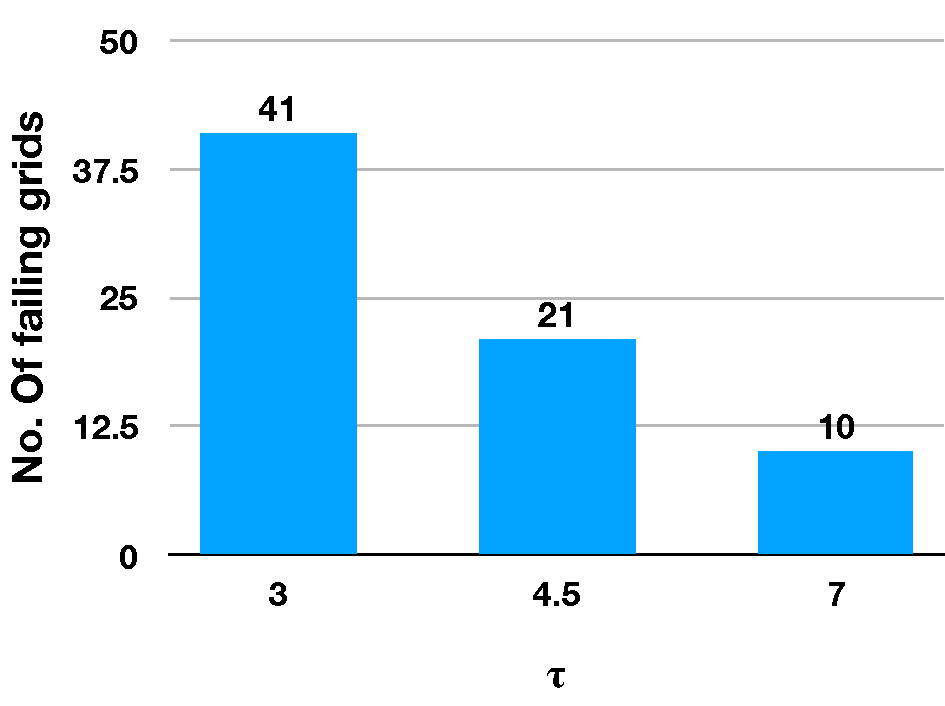
\includegraphics[scale=0.35]{Chapter4/fig/tvla.pdf}
\caption{Figure showing the number of failing regions with respect to $\tau$. It can be seen that it varies inversely with $\tau$.}
\label{fig:runtime}
%\vspace{-10pt}
\end{figure}

{\flushleft \em Runtime Analysis.} Each iteration of the {\em while} loop requires one trace collection step  to compute the TVLA in Line 1 and Line 5 of the algorithm. This trace collection takes up major portion of the run time. Besides this, the run time for the rest of {\sf Karna} is considerably small and is influenced mainly by the size of $\mathbb W$, the number of regions, and the security parameter $\tau$. 
A large value of the target delay $D$ implies that a large number of gates get added to $\mathbb W$ in Line 7 of Algorithm~\ref{alg:naive}. Similarly, a small value of $\tau$ indicates more number of regions failing (as seen in Figure~\ref{fig:runtime}), which in turn increases the size of $\mathbb W$. 
A  large value of the grid size will increase the run time as the number of regions that need to be checked in Line 4-5 of Algorithm~\ref{alg:naive} increases. 

Other factors that influence the run time are the number of local and global validations performed in Algorithm~\ref{alg:naive}. For each global validation, an STA call is made in Line 29 of Algorithm~\ref{alg:naive}. A full blown STA would have a run time complexity of $\mathcal{O} ( G^{2})$ where $G$ is the total number of gates in the design. In order to reduce the rum time, incremental Static Timing Analysis models such as the one used in~\cite{hu:12} or adaptive lazy timing analysis techniques like~\cite{MLTimer} can be employed. 

%\vspace{-3pt}
%The size of $\mathbb W$ also determines the termination 






%\todo{Factors influencing solution quality, runtime and factors influencing termination}
%which would cause only a minimal increase in the area. From our experiments, we observed that while the overall area remained constant, the area utilization increased.


%However, reconfiguring each gate with its low power equivalent will increase the delay of that particular gate. {\sf Karna} ensures that the reconfiguration doesn't violate the delay constraint by first checking if the gate has sufficient positive slack to undergo the reconfiguration (Line 22) and also perform Static Timing Analaysis on the design to ensure that the arrival time and required time constraints at all end-points are met (Line 30). It should be noted that though this timing analysis is a costly procedure, it ensures that the delay constraints are not violated. 

%The next configuration for each gate is chosen from the list P which consists of all the possible configurations sorted in increasing order. The algorithm traverses this list from right to left iteratively 
% We make use of Observation 3  (Section~\ref{sec:motivation}), i.e.,
% tuning gate parameters such as $V_{dd}$, $V_t$, and size can influence the side-channel leakage from the gate.
% In this step, we focus on optimizing the gate parameters such that the overall security of the design improves while the design parameters like area, power and delay remain unaffected.
% We use the Algorithm~\ref{alg:naive} for optimizing these gate parameters. The algorithm takes as input the synthesized netlist, the target frequency $F$ and, a standard cell library containing multiple cells with different $V_{dd}$, different threshold voltages $V_t$ and sizes for every gate. The netlist is represented as a Directed Acyclic Graph where the gates are represented by the nodes in the graph and the edges represent interconnects. The set of gates belonging to the vulnerable grids are stored in an array A.

% The algorithm works as follows, the gates are sorted in descending order based on their TVLA scores. The gate with the highest score i.e, the gates that are the most vulnerable in the design are the beginning of the list and the gates that are least vulnerable are the end. The algorithm then iteratively tries to optimize the $V_{dd}$, $V_{t}$ and size of each gate. The algorithm then checks for delay violations and commits the change if the proposed optimization doesn't violate the available delay budget of the gate. We then run a timing analysis to check if the proposed change causes any timing violations and undo the change if there are any such violations.

% It should be noted that this method is expensive in terms of runtime as the timing analysis procedure needs to be run for each and every gate in the array A. In order to speedup the optimization process we use the procedure reported in~\cite{MLtimer}. We define the set of gates that can be replaced in each iteration as the gate\_reconfiguration\_window $r$. Figure~\ref{fig:state-machine-window-sizing} and the value of $r$ at the end of every timing update is given in Table~\ref{tab:window-sizing-strategy}. It can be observed from this transition diagram that $state$ in timing update $i$ can be represented as $S_{v_{i-1}},v_i$, where $v_{i-1}$ and $v_i$ are binary digits that denote the stats of $(i-1)^{th}$ and $i^{th}$ timing updates respectively. A status of $v=0$ indicates a timing violation while a $1$ denotes a successful timing update. 
% We initialize $r$ to 2 and incrementally update the value of $r$ depending on the $state$ of the timing update. We limit the maximum value of $r$ to $\frac{N}{2}$, where $N$ stands for the total number of gates in the design. For example, if there is a timing violation in iterations $(i-1)$ and $i$ then the value of $r$ is set to 1 and the $state$ is set to 00, and only one gate is updated in the next iteration $(i+1)$, and if in the $(i+1)^{th}$ iteration there is no timing violation then the $state$ variable is updated to 01 and the value of $r$ is set to $r(i)*2$ ( 2 in this case as only one gate was replaced in the $i^{th}$ iterataion) and $r(i)*2$ gates are analyzed in the current iteration. Thus, the algorithm adaptively varies the window size depending on the $state$ variable.
% We sum up each iteration of the algorithm in the following steps.
% \begin{itemize}
 

% \item For each gate in the list A sort the gates based on the TVLA scores.

% \item For the first $r$ choices of A\; perform the following steps\;
% 	\begin{itemize}
%       \item if the gate has sufficient positive slack, we then replace the gate with the next configuration.
%     \end{itemize}

% \item We then check for any timing violations by running Static Timing Analysis. 

% \item If there is any delay violation, undo all reconfigurations.
% \begin{itemize}
% \item if $r$ is 1, then mark the corresponding gate as critical so that it cannot participate in any further timing optimizations.
% \item Update state and compute the new value of $r$.
% \end{itemize}
% \item  If timing evaluation is successful
% \begin{itemize}
% 	\item Run TVLA estimation, sort the gates based on updated TVLA values.
%     \item Update $state$ and compute the new value of $r$.
%     \item if value of $r$ is greater than A, the we resize $r$ to $\frac{A.size}{2}$.
% \end{itemize}

% \end{itemize}

%\item
%At the end of each iteration, {\sf Karna} checks the netlist for slew and capacitance violations. We incrementally upsize each gate in order to fix them. %Figure~\ref{fig:karna}
%shows the working of the {\sf Karna} module. 
%\end{itemize}
 
 
%Figure~\ref{fig:aesopt} showed that not all regions in the chip have a uniform TVLA value. In this step, we identify and optimize the gates in such vulnerable regions of the netlist. %It can be seen that for any given input, the amount of switching activity is different for different areas of the design. The side-channel leakage could be due to some areas of the design switching at a different rate for a specific input when compared to a random input.%Hence, in order to reduce the side-channel leakage  the gates belonging to these vulnerable areas need to be optimized. 
%In this step, we identify and optimize the gates in such vulnerable regions of the netlist.


 
 
 
 
% {\sf Karna} tries to achieve security without violating the design requirements. However, as mentioned earlier choosing gate configurations that favour security might violate the delay or area constraint. Hence, {\sf Karna} tries to balance between these two requirements.  It should be noted that the size of a region determines the nature of optimizations performed by {\sf Karna}. For example, consider the scenario where the value of $N$ is set such that there is only one gate per region. In this scenario {\sf Karna} would be able to identify uniquely the set of gates violating the secuirty constraints and change their configuration. This might cause the algorithm to select choices that are locally optimal i.e, they improve the overall security of the design but 
 
 
 
% While a high value of $N$ aggressively optimizes the design for security even at the cost of area and delay, a very low value would perform a lazy security optimization. For instance, when $N_{grids}=1$, the entire design is considered as a whole during the optimization process. This means that the algorithm might select gates that 
 
 
 %assessed for TVLA compliance. If it fails the TVLA test, all the gates belonging to the design are added to the working set of gates that needs to be optimized. This may lead to performance issues for designs that have a large number of gates. On the contrary, when $N_{grids}$ is equal to the number of gates in the design, each gate is checked for TVLA compliance and only the vulnerable gates are optimized. While this approach reduces the number of gates in the working set, this is also sub-optimal since the TVLA test has to be run for every gate in the design. More importantly, the algorithm may disregard placement dependencies between grids (i.e., delay and area budget of the design as a whole) since each grid is optimized in an isolated manner. Therefore, there is a need to select an optimal value of $N_{grids}$.

%A very high value of $N_{grids}$ will perform a fine-grained security analysis on the design while a low value of $N_{grids}$ will perform a coarse-grained analysis. For instance, setting $N_{grids}$ to the number of gates in the design will calculate the TVLA score for each gate in the netlist and identify if it is vulnerable, while a value of 1 will analyze the entire design as a whole and add all the gates to the vulnerable list. Thus the value of $N_{grids}$, much like the \texttt{-security\_level} option lets the designer specify the level of security expected from the design. A high value of $N_{grids}$ coupled together with a very low TVLA threshold would set extremely high security constraints on the design. Once the netlist is divided, the TVLA score is then calculated for each grid in the netlist. All the grids that do not comply with the TVLA score specified in the \texttt{-security\_level} option are marked as \textbf{unsafe} and the gates that belong to these grids are added to a working set. We then carefully tune the gate parameters of all the gates in this set in the next step, in order to improve the security of the design.


%{\flushleft \bf Reconfiguring the unsafe areas}
